\chapter{Эксперименты, ограничения, обсуждение} \label{chaptEval}

Завершаемость и корректность предложенного алгоритма формально доказаны выше, однако его производительность требует экспериментальной оценки. При этом основной интерес представляет оценка на входных данных, близких к реальным. Также требуется оценить предложенную архитектуру и реализующую её платформу. Вместе с этим необходимо рассмотреть границы применимости полученных в работе результатов. Таким образом, в данной главе решаются следующие задачи.

Оценка производительности проводилась на реальных и на синтетических данных. Краткое описание экспериментов приведено в таблице~\ref{tbl:PerfEval}.

\begin{table} [h]
  \centering
  \parbox{15cm}{\caption{Эксперименты по оценке производительности алгоритма синтаксического анализа динамически формируемых программ}\label{tbl:PerfEval}}
  \begin{tabular}{| p{6cm} | p{9cm}l |}
  \hline                               
  \hline
  Эксперимент & Что исследовалось & \\
  \hline
  \hline 
  Измерения на промышленном проекте                         & Особенности реальных входных данных, времени работы на реальных данных & \\
  \hline
  Измерение производительности на синтетических данных                         & Зависимость времени работы от структуры и размера входных данных & \\
  \hline
  Сравнение производительности с другими реализациями аналогичных алгоритмов   & Время работы на одинаковых входных данных &  \\
  \hline
  \hline
  \end{tabular}
\end{table}

Краткое описание экспериментов по оценке предложенной в работе архитектуры и реализующей её платформы представлено в таблице~\ref{tbl:ArchEval}.

\begin{table} [htbp]
  \centering
  \parbox{15cm}{\caption{Эксперименты по оценке архитектуры YC.SEL.SDK}\label{tbl:ArchEval}}
  \begin{tabular}{| p{6cm} | p{9cm}l |}
  \hline                               
  \hline
  Эксперимент & Что исследовалось & \\
  \hline 
  \hline
  Разработка синтаксического анализатора в промышленном проекте & Заменяемость компонент платформы на сторонние, реализованные ранее без использования платформы. & \\
    \hline
  Разработка расширений для Microsoft Visual Studio IDE         & Переиспользуемость компонент при разработке нескольких однотипных инструментов на основе предложенной платформы. Функциональные возможности инструментов, разработанных на основе платформы. & \\
  \hline
  \hline
  \end{tabular}
\end{table}

Далее приводятся детальные описания экспериментов и их результатов.


\section{Апробация в промышленном проекте по реинжинирингу}

Реализованный инструментарий был апробирован в рамках промышленного проекта ``S2O'' по миграции базы данных с MS-SQL Server 2005 на Oraclе 11gR2 компании ЗАО ``Ланит-Терком''.

Система состояла из 850 хранимых процедур и содержала около 2,6 миллионов строк кода на T-SQL. В ней имелось 2430 точек исполнения динамических запросов, из которых больше 75\% могли принимать более 
одного значения, а при их формировании использовалось от 7 до 212 операторов. При этом в среднем использовалось 40 операторов для формирования запроса~\cite{Syrcose}.

Так как анализатор языка T-SQL был разработан ранее в рамках проекта, в котором происходило внедрение, то для создания анализатора встроенного SQL была использована готовая грамматика и по ней построен 
синтаксический анализатор. Построение регулярной аппроксимации и лексический анализ также были реализованы ранее в рамках основного проекта и были переиспользованы. Возможность комбинирования сторонних компонент 
и компонент, созданных на основе YC.SEL.SDK, показало преимущества разделения шагов анализа.

Далее были реализованы функции вычисления метрик и вывода результата, после чего полученная функциональность была встроена в существующую цепочку обработки основного кода. В результате работы реализованных функций формировался отчёт, пример которого приведён в таблице~\ref{tbl:metrics}.

Тесты проводились на вычислительном устройстве с параметрами, эквивалентными указанным в разделе~\ref{SyntTestsEvalDescr}. В ходе экспериментов измерялись следующие характеристики для каждой точки выполнения динамически формируемого запроса.

\begin{itemize}
  \item Время обработки t в миллисекундах. Проводилось 10 запусков, время анализа усреднялось. 
  \item Размер входного конечного автомата: количество состояний \#Q и количество переходов \#T.
  \item Размер построенного SPPF: количество вершин \#V и количество рёбер \#E.
  \item Результат анализа: $'+'$ --- завершился успешно, $'-'$ --- завершился с ошибкой, T --- завершён по таймауту.
\end{itemize} 


\begin{table} [htbp]
  \centering
  \parbox{14cm}{\caption{Распределение динамически формируемых SQL-запросов по времени обработки}\label{tbl:timing}}
  \begin{tabular}{| p{8cm} || p{3cm} | p{3cm}l |}
  \hline                               
  \hline
  Категория динамически формируемых запросов&\centering Количество запросов &\centering Время обработки (минуты) & \\
  \hline 
  Содержат корректные выражения                  &\centering  2188         &\centering  14& \\
  Не содержат ни одного корректного выражения    &\centering  240          &\centering  9& \\
  Обработка завершена по таймауту                &\centering  1            &\centering  4&  \\
  \hline
  \textbf{Всего}                                 &\centering \textbf{2430} &\centering \textbf{27} & \\
  \hline
  \hline
  \end{tabular}
\end{table}

Результаты измерений времени работы представлены в таблице~\ref{tbl:timing}. Алгоритм успешно завершил работу на 2188 входных графах, аппроксимирующих множества значений запросов. Ручная проверка входных графов, на которых алгоритм завершался с ошибкой, показала, что они действительно содержали некорректные выражения. Причиной этого стала либо некорректная работа лексического анализатора, либо наличие в выражениях конструкций, не поддержанных в существующей грамматике. Так как лексический анализатор и грамматика были полностью заимствованы из оригинального проекта, то наличие этих ошибок не является недоработками алгоритма синтаксического анализа. Общее время синтаксического анализа составило 27 минут, из них 13 минут было затрачено на разбор графов, не содержащих ни одного корректного выражения. Из них 4 минуты --- обработка одного графа (5747 рёбер и 3897 вершин), прерванная по таймауту. Дальнейшие значения приводятся только для графов, которые удалось проанализировать. 604 из этих графов порождали ровно одно значение и анализировалось не более 1 миллисекунды. На разбор 1790 графов ушло не более 10 миллисекунд. На анализ двух графов было затрачено более 2 минут. Первый граф содержал 2454 вершин и 54335 рёбер, второй~--- 2212 вершин и 106020 рёбер. Распределение входных графов по промежуткам времени, затраченных на анализ, приведено на графике на рисунке~\ref{distr}.

\begin{figure}[H]
  \centering
 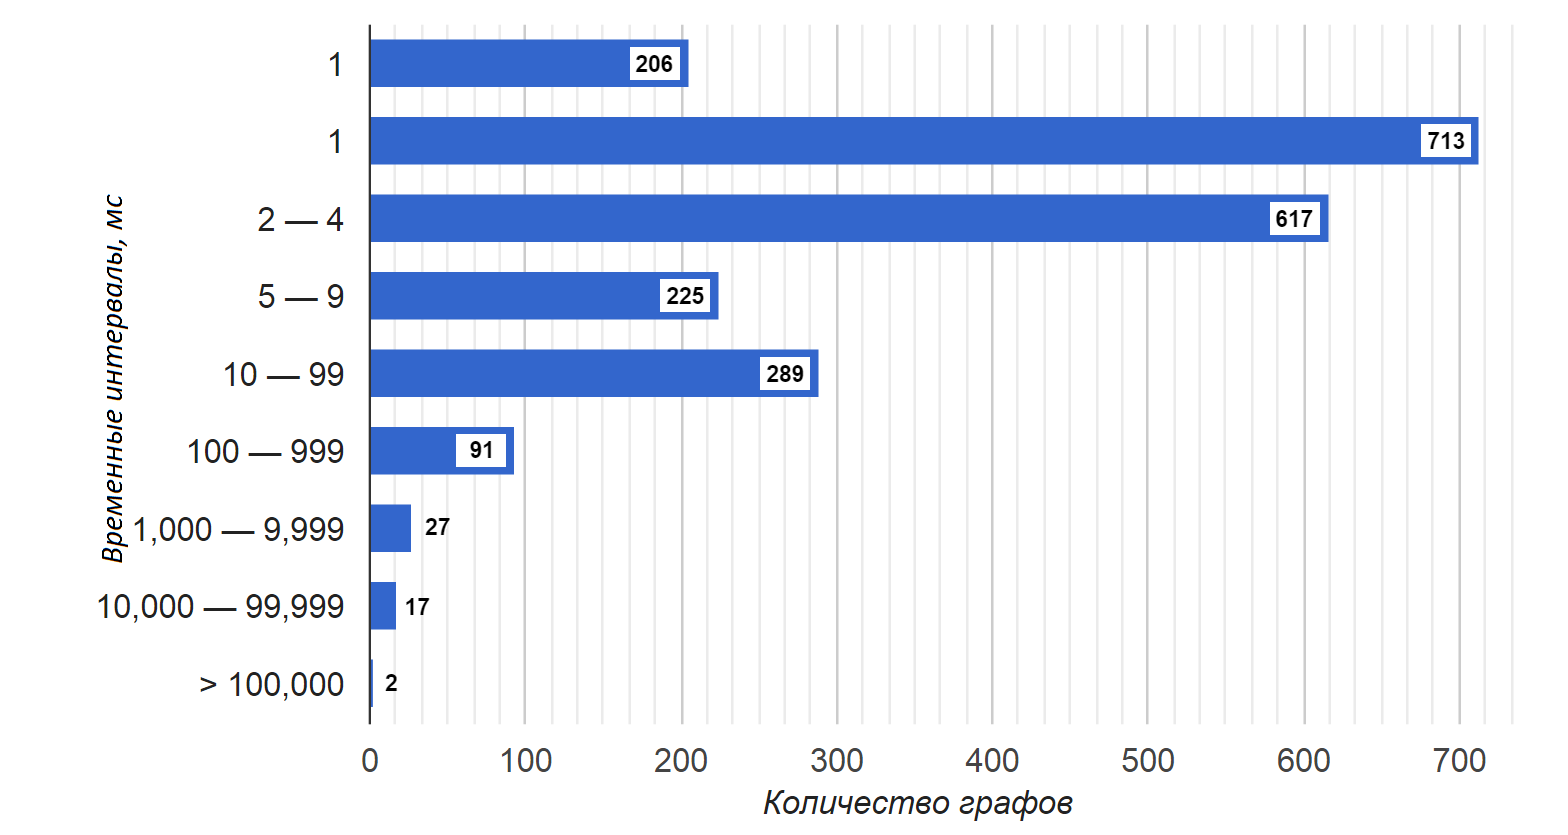
\includegraphics[width=0.95\textwidth]{pics/distr.png}
 \caption{Распределение запросов по времени анализа}
 \label{distr}
\end{figure}


\begin{table} [htbp]
  \centering
  \parbox{13cm}{\caption{Пример отчёта по результатам запуска синтаксического анализа в проекте ``S2O''}\label{tbl:metrics}}
  \begin{tabular}{| r | c | c | c | c | c | c |}
  \hline                               
  \hline
  \multirow{2}{*}{\textnumero} &\multirow{2}{*}{t(мс)} &\multirow{2}{*}{r} &\multicolumn{2}{c}{Размер DFA} &\multicolumn{2}{|c|}{Размер SPPF} \\
  \cline{4-7} 
                               &                   &                   & \hspace{8pt}~\#Q~~~~     & ~~\#T~~          & \#V         &         \#E \\ 
  \hline 
1  &6      &$+$ &75  &76      &1074    &1075      \\
2  &73     &$+$ &104 &806   &18786   &26377   \\
3  &64     &$+$ &79  &750     &17237     &23954   \\
4    &15982  &$+$ &817 &32281 &920618    &1885112   \\
5    &3      &$+$ &108 &107   &996     &995     \\
6    &256000 & T  &3897&5747  &0       &0         \\
7    &28360  &$+$ &924 &41408 &1315491 &2794517 \\
8    &17     &$+$ &236 &506   &4608    &5165      \\
9    &207    &$+$ &928 &2249  &38709     &57352   \\
10 &110    &$+$ &390 &942     &14757     &21805   \\
11 &111    &$+$ &377 &967     &14812     &21902   \\
12 &262    &$+$ &764 &1907  &33332   &49955   \\
13 &3      &$+$ &117 &116     &1093      &1092    \\
14 &3      &$+$ &92  &92      &1391    &1391      \\
  \hline
  \hline

  \end{tabular}
\end{table}



Тестирование на реальных данных показало, что предложенный в работе алгоритм синтаксического анализа применим в промышленных проектах. Также данная апробация показала, что предложенная архитектура SDK позволяет использовать отдельные компоненты независимо и комбинировать их.

\section{Экспериментальная оценка производительности алгоритма}\label{SyntTestsEvalDescr}

Алгоритм синтаксического анализа динамически формируемых выражений был протестирован на нескольких наборах синтетических тестов, цель которых заключалась в исследовании производительности алгоритма на практически значимых входных данных. Анализ  проекта ``S2O'' показал, что запросы часто формируются конкатенацией фрагментов, каждый из которых формируется с помощью ветвлений или циклов. Ниже приведена эталонная грамматика $G_t$, использованная в этих тестах.

$$
\begin{array}{crcl}
& start\_rule &::=& s \\
& s & ::= & s \mbox{\texttt{ PLUS }} \mbox{\texttt{n}}\\
& n & ::= & \mbox{\texttt{ONE | }} \mbox{\texttt{TWO | }} \mbox{\texttt{THREE | }} \mbox{\texttt{FOUR | }} \\
&   &     & \mbox{\texttt{FIVE | }} \mbox{\texttt{SIX | }} \mbox{\texttt{SEVEN}}
\end{array}
$$

Входные данные представляли собой конечные автоматы над алфавитом терминальных символов грамматики $G_t$, построенные с помощью конкатенации базовых блоков. Предполагается, что такие графы могут быть получены в результате лексического анализа регулярной аппроксимации, построенной по некоторой программе. В данном случае базовый блок --- это шаблонный конечный автомат, который используется для построения тестовых конечных автоматов. Каждый пакет тестов характеризовался тремя параметрами: 

\begin{itemize}
  \item $height$~--- количество ветвлений в базовом блоке;
  \item $length$~--- максимальное количество повторений базовых блоков;
  \item $isCycle$~--- наличие в базовом блоке циклов (если значение равно \texttt{false}, то используются базовые блоки, изображённые на рисунке~\ref{block}, если \texttt{true}~--- то изображённые на рисунке~\ref{block_loop}).
\end{itemize}

\begin{figure}[h!]
 \centering
 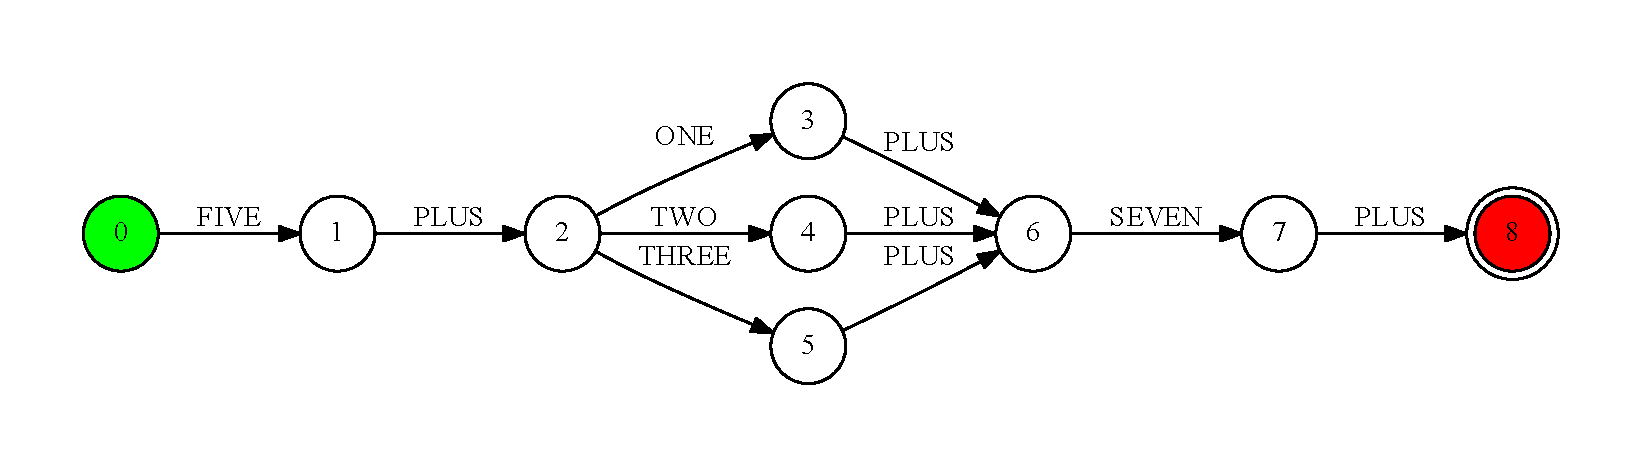
\includegraphics[width=15cm]{pics/block.pdf}
 \caption{Базовый блок без циклов при $height=3$}
 \label{block}
\end{figure}

\begin{figure}[h!]
 \centering
 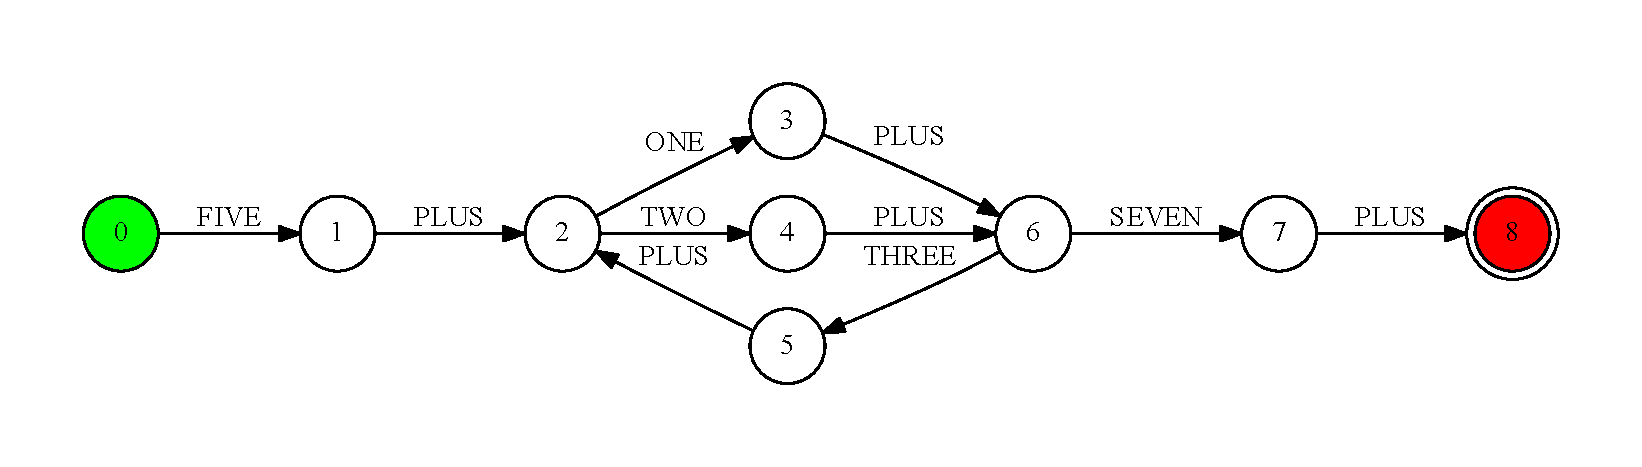
\includegraphics[width=15cm]{pics/block_loop.pdf}
 \caption{Базовый блок, содержащий цикл, при $height=3$}
 \label{block_loop}
\end{figure}

Замеры проводились на вычислительной станции со следующими характеристиками.
\begin{itemize}
\item Операционная система: Microsoft Windows 8.1 Pro.
\item Тип системы: x64-based PC.
\item Процессор: Intel(R) Core(TM) i7-4790 CPU @ 3.60GHz, 3601 Mhz, 4 Core(s), 8 Logical Processor(s).
\item Объём оперативной памяти: 16.0 GB.
\end{itemize}

Чтобы выявить зависимость времени работы алгоритма от размера входных данных, были созданы пакеты из $500$ тестов. Все тесты в каждом из пакетов содержали одинаковое количество ветвлений в базовом блоке. 
При этом количество повторений блока совпадает с порядковым номером теста, то есть $length=i$ для $i$-того теста. Для каждого теста измерялось время, затраченное на синтаксический анализ. Измерения проводились 
10 раз, после чего вычислялось среднее время обработки одного графа. График, представленный на рисунке~\ref{diffheights}, иллюстрирует зависимость времени, затрачиваемого на синтаксический анализ, от количества повторения базового блока и количества ветвлений в каждом из них. Можно заметить, что время растёт линейно в зависимости от размера входного графа. График на рисунке~\ref{CycleVsLinear} показывает, что 
наличие циклов в графе при одинаковом значении параметра $height$ увеличивает продолжительность анализа, зависимость времени от размера графа остаётся линейной.

\begin{figure}[h!]
 \centering
 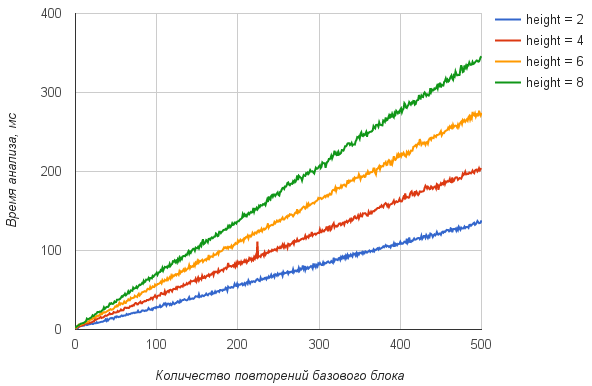
\includegraphics[width=15cm]{pics/diffheights.png}
 \caption{Зависимость времени работы алгоритма от размера входного графа при $isCycle=false$}
 \label{diffheights}
\end{figure}

\begin{figure}[h!]
 \centering
 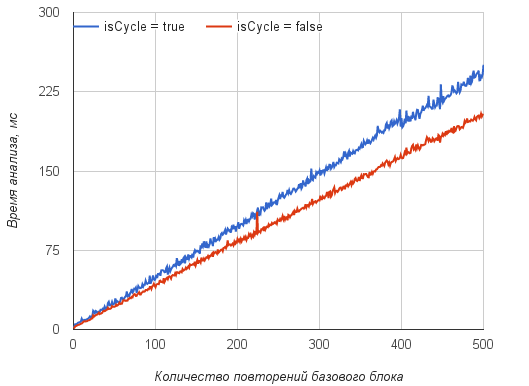
\includegraphics[width=13cm]{pics/heigh4.png}
 \caption{Зависимость времени работы алгоритма от размера входного графа и наличия в нем циклов при $height=4$}
 \label{CycleVsLinear}
\end{figure}


\section{Сравнение с инструментом Alvor}

Единственным доступным для сравнения инструментом, производящим синтаксический анализ динамически формируемого кода, является Alvor~\cite{Alvor1, Alvor2}. Другие инструменты либо основаны на других подходах и решают другие задачи (например, \cite{JSA,PHPSA}), либо отсутствуют в открытом доступе (например, инструмент описываемый в работах~\cite{LrAbstract1,LrAbstract2}). Alvor реализует  близкий к представленному в работе подход: независимые шаги анализа, что позволяет легко выделить синтаксический анализ, который основан на GLR-алгоритме. Существенным отличием от разработанного алгоритма является то, что Alvor не строит деревья вывода. Исходный код Alvor опубликован~\cite{AlvorUrl}, что позволяет модифицировать его таким образом, чтобы измерять параметры выполнения конкретных методов. 

Сравнение производилось на синтетических тестах, которые строились по принципу, аналогичному изложенному в разделе~\ref{SyntTestsEvalDescr}. Так как Alvor на вход принимает регулярное выражение, называемое \textit{абстрактной строкой}~\cite{Alvor2}, а анализатор, созданный на основе YC.SEL.SDK --- конечный автомат, то был реализован генератор, который по входным параметрам создает файл с абстрактной строкой и с описанием соответствующего автомата в формате DOT~\cite{DOT}. Синтаксис описания абстрактной строки приведён в листинге~\ref{lst:absStr}. При этом абстрактная строка подвергалась последовательно лексическому и синтаксическому анализу и измерялось время работы последнего, а конечный автомат строился сразу над алфавитом токенов и подвергался синтаксическому анализу.

\fvset{frame=lines,framesep=5pt}
\begin{listing}
    \begin{pyglist}[numbers=left,numbersep=5pt]
absStr = "str"
       | '{'absStr(',' absStr)+'}' //alternatives
       | absStr absStr             //concatenation
       | absStr '*'                //closure
\end{pyglist}
\caption{Синтаксис описания абстрактной строки}
\label{lst:absStr}
\end{listing}

 
Примеры тестовых входов для одинаковых входных параметров (однократного и двукратного повторения базовых блоков и $height=2$ ) для инструмента на YC.SEL.SDK и Alvor представлены на рисунке~\ref{fig:YCInput} и листинге~\ref{lst:AlvorInputEx}  соответственно. 

\fvset{frame=lines,framesep=5pt}
\begin{listing}
    \begin{pyglist}[numbers=left,numbersep=5pt]
"select "{"X3 + Y4","1"}",d from tbl"
"select "{"X3 + Y4","1"}","{"X7 + Y8","5"}",d from tbl"
\end{pyglist}
\caption{Пример абстрактных строк для $height=2$ одного и двух повторений базового блока}
\label{lst:AlvorInputEx}
\end{listing}

\begin{figure}[h!]
 \centering
 \includegraphics[width=0.98\textwidth]{pics/ycSQLinput.eps}
 \caption{Входной граф для синтаксического анализатора на базе YC.SEL.SDK при $height=2$ и двух повторениях базового блока}
 \label{fig:YCInput}
\end{figure}

Результаты измерений представлены в таблице~\ref{tbl:YCvsAlvor} и на рисунке~\ref{fig:YCvsAlvor}. В легенде и в заголовке таблицы указан инструмент (YC или Alvor) и значение параметра $height$ (например, h=2).

При более чем шестнадцатикратном повторении блоков с $height=2$ время работы Alvor превысило 30 минут и измерения были прекращены. Аналогичная ситуация возникает при более чем десятикратном повторении блоков с $height=3$. Таким образом, измерения показывают, что время работы анализатора Alvor растёт экспоненциально относительно количества повторений базового блока при $height>1$. Анализатор, созданный на основе YC.SEL.SDK, в таких случаях имеет лучшую производительность. При этом на линейном входе Alvor работает быстрее. Однако, асимптотика YC.SEL.SDK на входных данных, имеющих подобную структуру, такая же, как у оригинального алгоритма RNGLR, что показано в предыдущих экспериментах. При этом существуют возможности для оптимизации текущей реализации, благодаря чему производительность на линейном входе может быть улучшена.

\begin{figure}[h!]
 \centering
 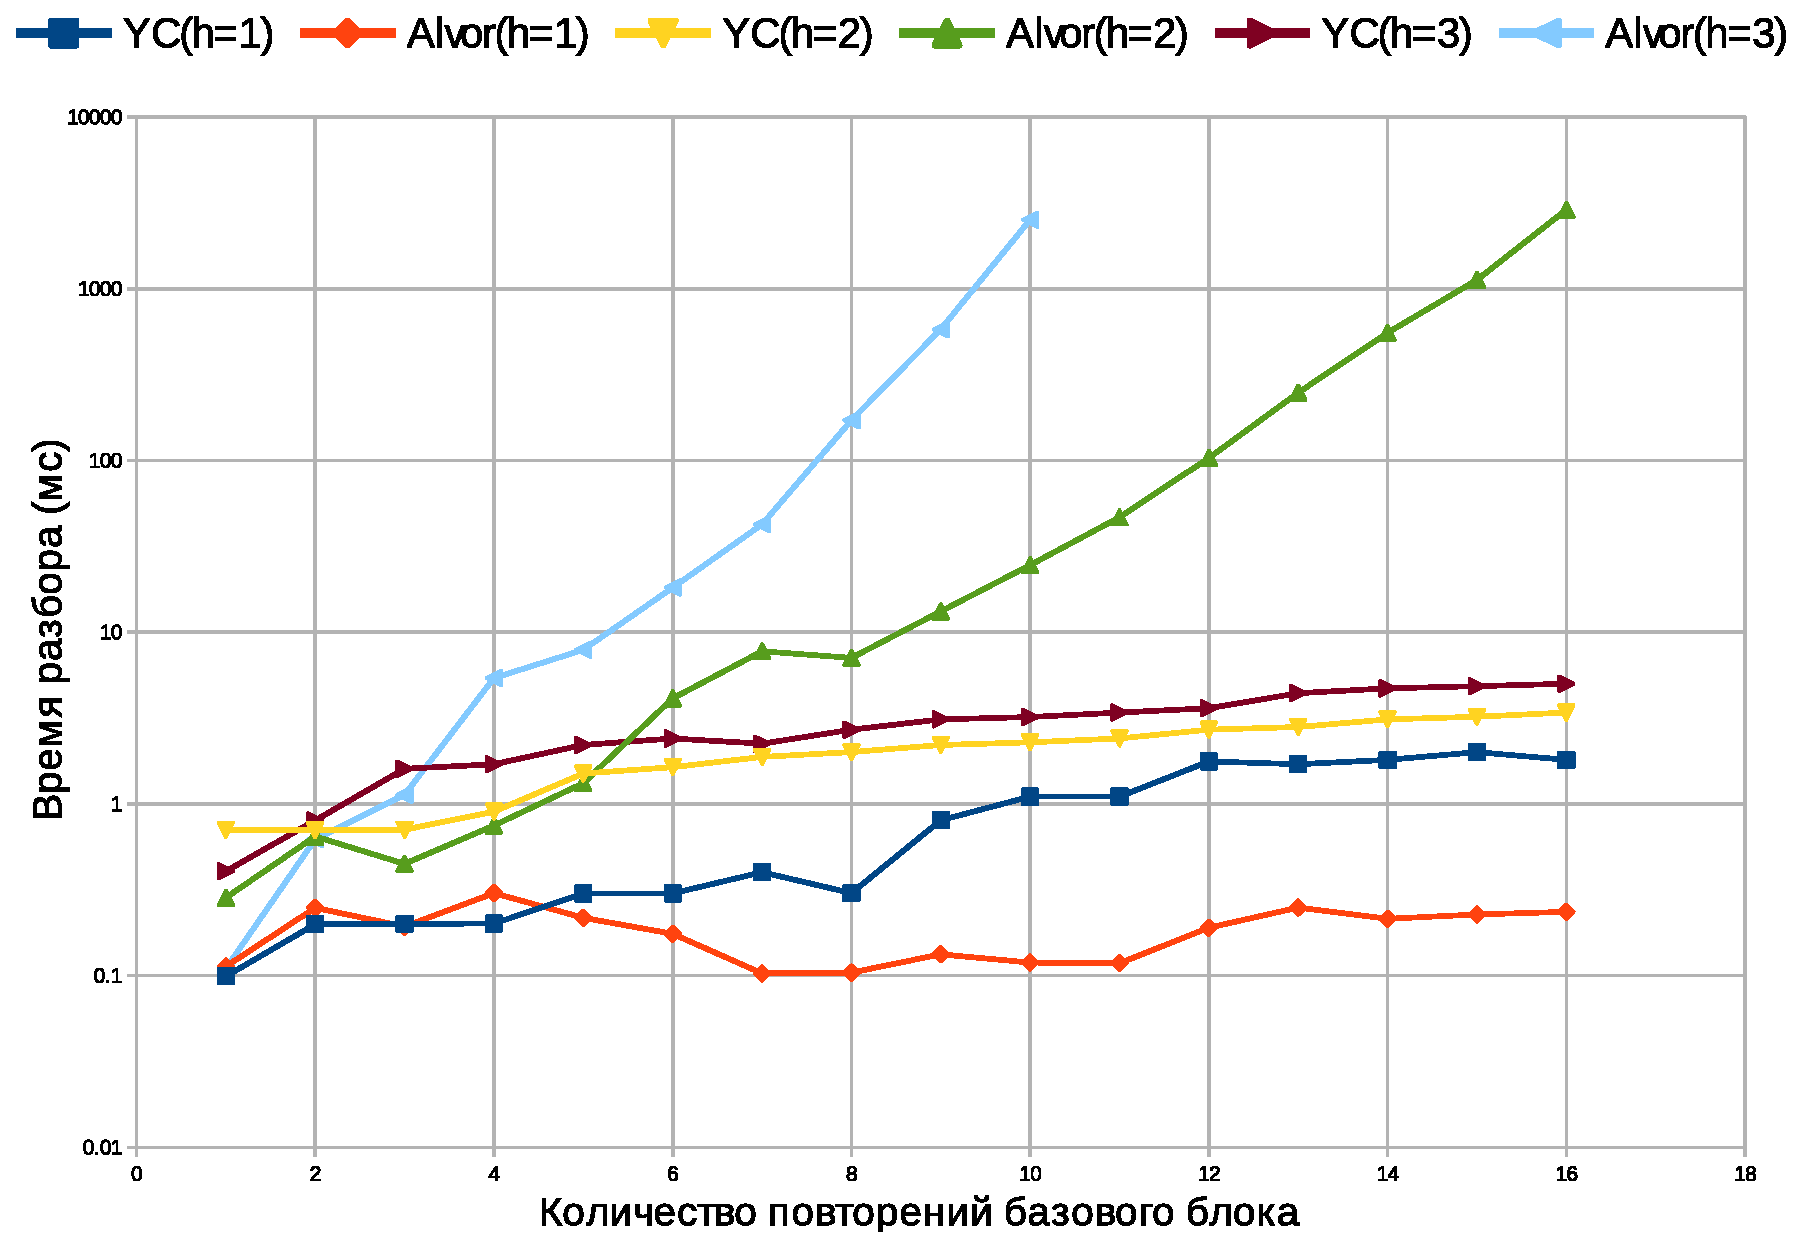
\includegraphics[width=0.95\textwidth]{pics/AlvorVsYC.eps}
 \caption{Сравнение производительности Alvor и синтаксического анализатора на базе YC.SEL.SDK}
 \label{fig:YCvsAlvor}
\end{figure}


\begin{table} [htbp]
  \centering
  \parbox{14cm}{\caption{Результаты сравнения производительности Alvor и синтаксического анализатора на базе YC.SEL.SDK}\label{tbl:YCvsAlvor}}
  \begin{tabular}{| c | c | c | c | c | c |}
  \hline                               
  \hline
  YC(h=1) & Alvor(h=1) & YC(h=2) & Alvor(h=2) & YC(h=3) & Alvor(h=3)\\
  \hline 
0.099 &  0.113 &  0.706 &  0.284   & 0.405 &  0.11     \\
0.199 &  0.248 &  0.702 &  0.646   & 0.801 &  0.622    \\
0.2   &  0.193 &  0.707 &  0.447   & 1.601 &  1.129    \\
0.201 &  0.302 &  0.901 &  0.748   & 1.701 &  5.403    \\
0.3   &  0.217 &  1.502 &  1.32    & 2.203 &  7.89     \\
0.301 &  0.175 &  1.635 &  4.114   & 2.402 &  18.187   \\
0.4   &  0.103 &  1.877 &  7.734   & 2.24  &  42.447   \\
0.302 &  0.104 &  2.002 &  7.076   & 2.704 &  171.529  \\
0.802 &  0.133 &  2.202 &  13.204  & 3.104 &  580.545  \\
1.102 &  0.119 &  2.282 &  24.578  & 3.204 &  2521.318 \\
1.102 &  0.118 &  2.404 &  46.662  & 3.403 &           \\
1.766 &  0.19  &  2.704 &  103.417 & 3.605 &           \\
1.701 &  0.249 &  2.803 &  248.107 & 4.408 &           \\
1.803 &  0.214 &  3.103 &  554.314 & 4.706 &           \\
2.001 &  0.227 &  3.217 &  1125.976& 4.843 &           \\
1.803 &  0.235 &  3.403 &  2886.261& 5.006 &           \\
  \hline
  \hline

  \end{tabular}
\end{table}

Так как Alvor не предоставляет платформы для простой реализации поддержки новых языков, то для сравнения было выбрано подмножество языка SQL, общее для Alvor и реализованного в рамках апробации инструмента. Отсутствие возможности быстро построить новый анализатор на основе Alvor помешало сравнению на реальных данных, так как спецификация грамматики T-SQL является задачей, требующей большого количества времени. По этой причине замеры производились на синтетических тестах. В результате измерений было выяснено, что производительность реализованного алгоритма синтаксического анализа лучше чем производительность аналогичного алгоритма, реализованного в инструменте Alvor на входных данных, содержащих большое количество ветвлений: Alvor показывает экспоненциальный рост времени обработки, а реализованный алгоритм является полиномиальным, что согласуется с результатами, полученными в предыдущем разделе.

\section{Разработка расширений для поддержки встроенных языков}

На основе YC.SEL.SDK и YC.SEL.SDK.ReSharper, представленых ранее, были реализованы расширения к ReSharper, которые предоставляют поддержку для  двух встроенных языков: подмножества языка T-SQL~\cite{TSQL} и языка арифметических выражений Calc. Реализация данных расширений также являлась апробацией предложенной архитектуры разработанного инструментального пакета.

В рамках данного шага апробации были созданы лексические спецификации и грамматики соответствующих языков (код опубликован в открытом доступе~\footnote{Репозиторий проекта YaccConstructor, содержащий набор различных грамматик (дата обращения: 29.07.2015): \url{https://github.com/YaccConstructor/YC.GrammarZOO}}). Далее, с помощью генераторов разработанного инструментария по этим грамматикам были построены синтаксические анализаторы, а по лексическим спецификациям --- лексические анализаторы.

При создании расширений был также апробирован механизм построения регулярной аппроксимации. Для построения графа потока управления внешнего вода использовалась функциональность ReSharper SDK. Затем полученный граф переводился в обобщённое представление, по которому строилась регулярная аппроксимация средствами разработанного инструмента.

После того, как отдельные части были готовы, они были объединены в готовый плагин на основе YC.SEL.SDK.ReSharper. В результате было получено два расширения, предоставляющие поддержку соответствующих языков и ядро, содержащее общую, независимую от языков функциональность, обеспеченивающую взаимодействие между ReSharper и реализованными расширениями.

Компоненты предоставляют подсветку синтаксиса (рисунок~\ref{fig:sHiglighting}) и подсветку парных элементов (рисунок~\ref{fig:braces}). Для языка Calc также реализована статическая диагностика семантических ошибок, а именно, поиск использования необъявленных переменных. Это показывает, с одной стороны, возможность непосредственного использования SPPF для проведения анализа динамически формируемого кода, а с другой --- возможность реализации дополнительной функциональности, не являющейся общей функциональностью SDK.

Результаты статического поиска использования необъявленных переменных показан на 
рисунке~\ref{fig:undeclaredVars}. В данном примере переменная \verb|x| объявляется в одной из веток условного оператора и не объявляется в другой, что может привести к ошибке в точке использования, о чём сообщается пользователю.

\begin{figure}[H]
  \centering
 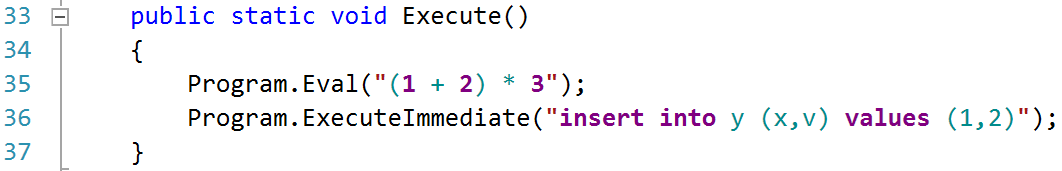
\includegraphics[width=0.95\textwidth]{pics/multilanguages_light.png}
 \caption{Пример подсветки синтаксиса для нескольких встроенных языков: SQL и Calc}
 \label{fig:sHiglighting}
\end{figure}

\begin{figure}[H]
 \centering
 \begin{subfigure}[b]{0.47\textwidth}
  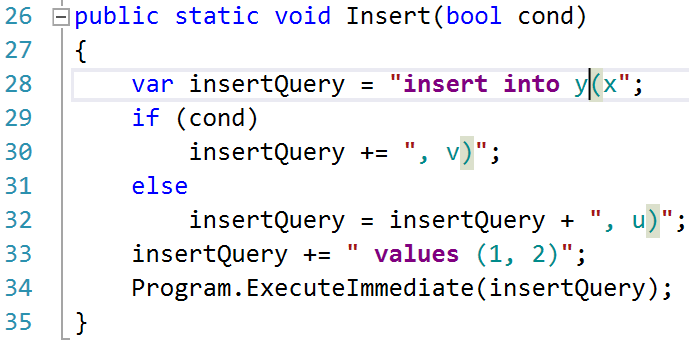
\includegraphics[width=\textwidth]{pics/brackets_one_to_many_light.png}
  \caption{Одной открывающей скобке соответствует несколько закрывающих}
  \label{fig:brOneToMany}
  \end{subfigure}
  ~
 \begin{subfigure}[b]{0.47\textwidth}
  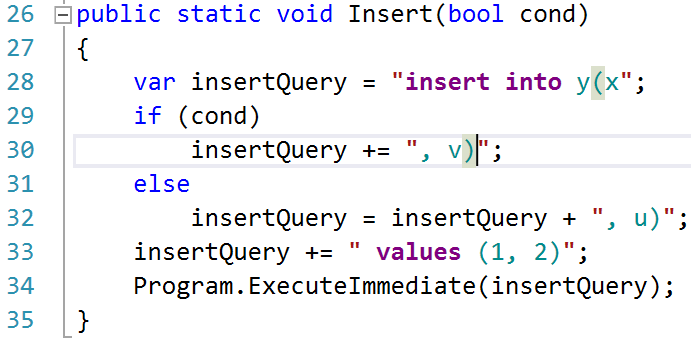
\includegraphics[width=\textwidth]{pics/brackets_one_to_one.png}
  \caption{Одной закрывающей скобке соответствует одна открывающая}
  \label{fig:brOneToone}
 \end{subfigure}

 \caption{Пример подсветки парных скобок}
 \label{fig:braces}
\end{figure}

\begin{figure}[H]
  \centering
 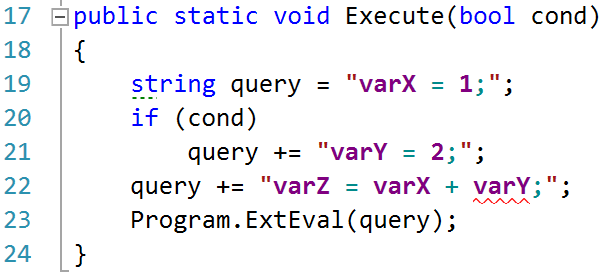
\includegraphics[width=0.65\textwidth]{pics/undefined_variable.png}
 \caption{Пример статического обнаружения семантических ошибок для языка Calc}
 \label{fig:undeclaredVars}
\end{figure}

\begin{figure}[H]
  \centering
 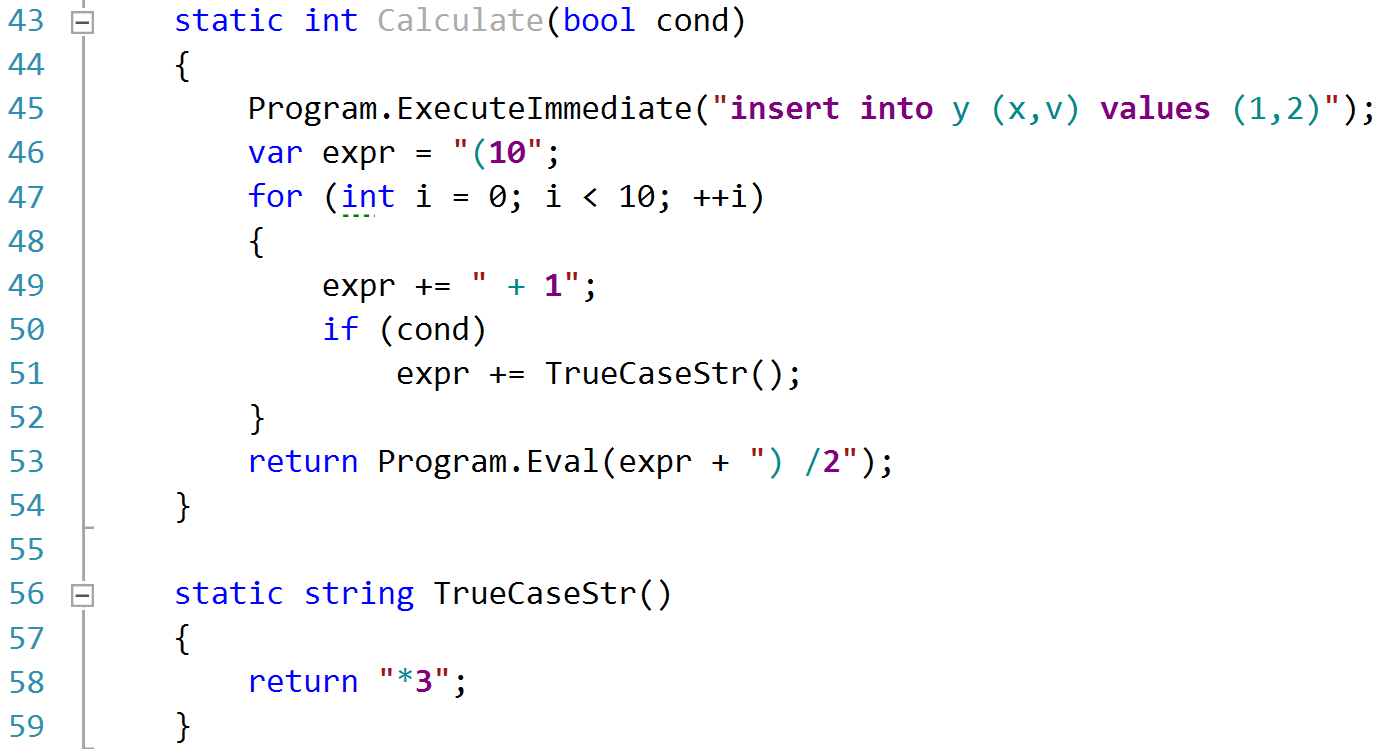
\includegraphics[width=0.95\textwidth]{pics/sql_calc_cycle.png}
 \caption{Пример межпроцедурной обработки встроенных языков}
 \label{fig:interProc}
\end{figure}

Расширения опубликованы в виде готовых к использованию бинарных пакетов. Функциональность, отвечающая за поддержку каждого языка, распространяется в виде самостоятельного бинарного пакета и может быть независимо подключена или отключена. Структура пакетов представлена на рисунке~\ref{fig:packagesStructure}. Пакет YC.SEL.Plugins.Core содержит функции, общие для обработки произвольных встроенных языков, что показывает возможность эффективного переиспользования при разработке однотипных инструментов. Пакеты YC.SEL.Plugins.Calc и YC.SEL.Plugins.TSQL содержат функции, необходимые для поддержки соответствующих языков. Они расширяют возможности ReSharper как непосредственно, так и через YC.SEL.Plugins.Core, используя общие функции.

\begin{figure}[H]
  \centering
 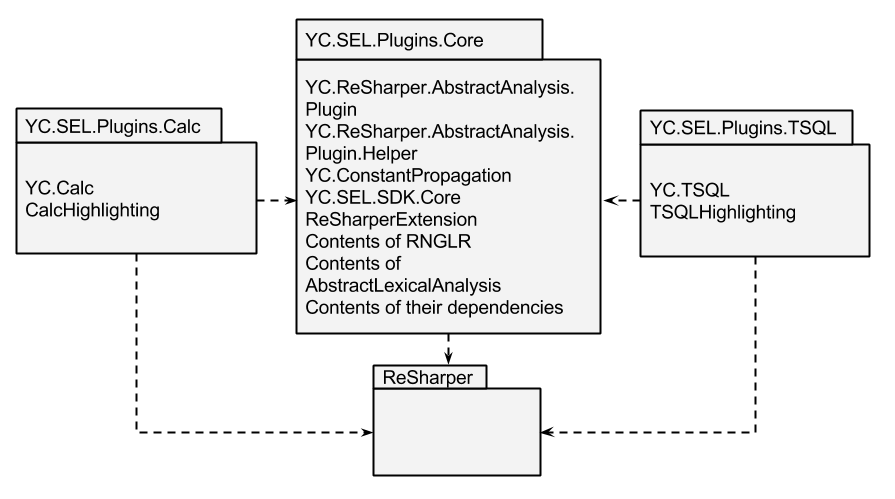
\includegraphics[width=0.90\textwidth]{pics/RshPluginsPackages.png}
 \caption{Структура пакетов расширений для ReSharper, предоставляющих поддержку встроенных T-SQL и Calc}
 \label{fig:packagesStructure}
\end{figure}

Дополнительно в результате разработки расширений было подтверждено, что независимость шагов обработки динамически формируемых выражений позволяет гибко переиспользовать компоненты, реализующие эти шаги. Например, анализаторы, разработанные в рамках расширений для ReSharper, используются в тестах, не связанных с ReSharper, то есть одни и те же анализаторы используются вместе с различными компонентами для построения аппроксимации.

\section{Ограничения}

Используемые подходы и алгоритмы накладывают ограничения на платформу и инструменты, разрабатываемые на её основе. Данный раздел посвящён обсуждению этих ограничений.

Множество, являющееся аппроксимацией значений динамически формируемого выражения, принимаемое на вход алгоритмом синтаксического анализа, должно быть регулярным. То есть аппроксимация задаёт регулярный язык, в то время как язык, генерируемый программой, может быть рекурсивно-перечислимым. Это означает, что за на этапе построения аппроксимации будет происходить потеря точности. Например, нехвостовая рекурсия невыразима в терминах регулярных множеств. Точность построения конкретной регулярной аппроксимации зависит от конкретного алгоритма, используемого для этих целей. Алгоритм может реализовывать или не реализовывать межпроцедурный анализ, поддерживать или не поддерживать строковые операции, разными способами обрабатывать пользовательский ввод и другие ситуации, когда значение выражения вычислить невозможно. Наш алгоритм поддерживает межпроцедурный анализ и строковые операции. 

Эталонный язык должен быть описан детерминированной контекстно-свободной грамматикой. Большинство языков программирования могут быть описаны такой грамматикой. Однако бывают исключения, например, язык C++. С другой стороны, в документации языка может быть приведена неоднозначная грамматика, а её приведение к детерминированной может потребовать значительных временных затрат. 

Вопросы быстродействия инструментов зависят от контекста их использования. Если при реинжиниринге время обработки кода не всегда является существенным фактором, то для многих инструментов, используемых  в средах разработки, время отклика критично.  Особенно это важно для функциональности, работающей в режиме ``на лету'': подсветка синтаксиса, автодополнение, подсказки. Так как платформа создавалась с ориентацией на разработку инструментов для реинжинирига, то некоторые компоненты направлены на увеличение точности анализа в ущерб производительности. Например, компонента построения регулярной аппроксимации гарантирующая построение приближения сверху, учитывает циклы и строковые функции~\cite{RegOverApprox}, что повышает точность анализа, однако производительность может оказаться слишком низкой для использования компоненты в средах разработки. С другой стороны, при создании инструмента для IDE возможно заменить алгоритм построения аппроксимации на более быстрый, но менее точный. Например в инструменте Alvor~\cite{Alvor2}, предназначенном прежде всего для интерактивной работы в среде разработки, предлагается именно такой алгоритм.  При этом важно, что возможности платформы позволяют комбинировать различные реализации компонент. То есть можно использовать один и тот же синтаксический анализатор с разными вариантами лексического для получения требуемых характеристик результирующего инструмента. С другой стороны, текущая реализация содержит возможности для различных оптимизаций, в частности, некоторые алгоритмы могут быть ускорены с помощью распараллеливания. Выбор оптимальных структур данных, например для конечных автоматов, активно использующихся в рамках платформы, является темой отдельного исследования~\cite{DataStructureForFA}.

В 2015 году была опубликована работа~\cite{SPPF2015}, являющаяся одной из первых, посвящённой систематическому исследованию работы с SPPF в контексте обобщённого синтаксического анализа. В рамках  анализа динамически формируемых выражений исследований в этом направлении не обнаружено. По этой причине в рамках данной работы реализован только прототип библиотеки, позволяющей решать некоторые задачи над SPPF в общем виде, например, поиск необъявленных переменных. Теоретическое исследование данного вопроса является отдельной задачей. С другой стороны, было доказано, что из построенного SPPF могут быть извлечены деревья вывода для любых цепочек из аппроксимации, а с деревьями можно работать с помощью стандартных методов. 

\clearpage

